\section{Similarity}

\textbf{General Equation:} Two polygons are similar if all corresponding sides are in proportion.

\vfill
\begin{enumerate}[labelindent=*,style=multiline,leftmargin=*,label=\textbf{Example \arabic*:}]
\item Square ABCD and square EFGH have side lengths in a ratio of $1:2$. What percentage increase is the area of EFGH to ABCD?

\vfill\item Line segment DE is drawn in triangle ABC so that D is the midpoint of AB and E is the midpoint of AC. What is the ratio of the areas of ADE to EDBC?

\vfill\item Two concentric circles are drawn such that the radius of the outer circle is twice the diameter of the inner circle. What percentage is the circumference of the outer circle to the circumference of the inner?
\end{enumerate}

\vfill
\newpage
\begin{multicols*}{2}
\begin{outline}[enumerate]
\medium

\1 The circumference of a children's basketball is 27.5 inches whereas the circumference of an NBA basketball is 29.5 inches. What is the ratio of their volumes?

\bigskip
\textbf{Equation/Strategy:} \hrulefill

\bigskip
\textbf{Solve:}

\vfill
\2 $55:59$
\2 $351:433$
\2 $351:434$
\2 $437:469$
\2 $438:470$

\midline

\1 An equilateral triangle is inscribed in another so that only the vertices of the inner triangle touch the edges of the outer. What is the greatest possible ratio of the area of the smaller triangle to the bigger one?

\bigskip
\textbf{Equation/Strategy:} \hrulefill

\bigskip
\textbf{Solve:}

\vfill
\2 $1:9$
\2 $1:4$
\2 $1:3$
\2 $1:2$
\2 $2:3$

\columnbreak
\advanced

\1 Right triangle BDC is similar to triangle ABC as shown below.

\begin{center}
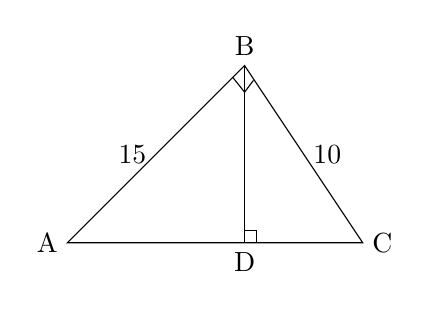
\begin{tikzpicture}[scale=0.75]
\draw (0,0) node[left] {A} -- (3,3) node[above] {B} node[midway,left] {15} -- (5,0) node[right] {C} node[midway, right] {10} -- cycle;
\draw (3,3) -- (3,0) node[below] {D};
\draw (3,0.2) -- (3.2,0.2) -- (3.2,0);
\draw (2.8,2.8) -- (3,2.55) -- (3.15,2.75);
\end{tikzpicture}
\end{center}

If AB = 15 and BC = 10, what is the length of BD?

\bigskip
\textbf{Equation/Strategy:} \hrulefill

\bigskip
\textbf{Solve:}

\vfill
\2 7.5
\2 8
\2 12.5
\2 $\frac{30\sqrt{13}}{13}$
\2 $150-\sqrt{325}$

\midline

\1 What is the ratio of the diagonal of the a cube with a volume of 8 cm$^3$ to the diagonal of a cube with a volume of 64 cm$^3$?

\bigskip
\textbf{Equation/Strategy:}

\bigskip
\textbf{Solve:}

\vfill
\2 $1:8$
\2 $1:4$
\2 $1:2$
\2 $\sqrt{2}:4$
\2 $\sqrt{2}:\sqrt{3}$
\end{outline}
\end{multicols*}